% --------------------------------------------------------------
% This is all preamble stuff that you don't have to worry about.
% Head down to where it says "Start here"
% --------------------------------------------------------------
 
\documentclass[12pt]{article}
 
\usepackage[margin=1in]{geometry} 
\usepackage{amsmath,amsthm,amssymb}
 
\newcommand{\N}{\mathbb{N}}
\newcommand{\Z}{\mathbb{Z}}
 
\newenvironment{theorem}[2][Theorem]{\begin{trivlist}
\item[\hskip \labelsep {\bfseries #1}\hskip \labelsep {\bfseries #2.}]}{\end{trivlist}}
\newenvironment{lemma}[2][Lemma]{\begin{trivlist}
\item[\hskip \labelsep {\bfseries #1}\hskip \labelsep {\bfseries #2.}]}{\end{trivlist}}
\newenvironment{exercise}[2][Exercise]{\begin{trivlist}
\item[\hskip \labelsep {\bfseries #1}\hskip \labelsep {\bfseries #2.}]}{\end{trivlist}}
\newenvironment{problem}[2][Problem]{\begin{trivlist}
\item[\hskip \labelsep {\bfseries #1}\hskip \labelsep {\bfseries #2.}]}{\end{trivlist}}
\newenvironment{question}[2][Question]{\begin{trivlist}
\item[\hskip \labelsep {\bfseries #1}\hskip \labelsep {\bfseries #2.}]}{\end{trivlist}}
\newenvironment{corollary}[2][Corollary]{\begin{trivlist}
\item[\hskip \labelsep {\bfseries #1}\hskip \labelsep {\bfseries #2.}]}{\end{trivlist}}

\newenvironment{solution}{\begin{proof}[Solution]}{\end{proof}}

\usepackage{lipsum}
\usepackage[colorlinks=true, linkcolor=blue, citecolor=blue, urlcolor=blue]{hyperref}
\usepackage{cleveref}
\usepackage{graphicx}
\usepackage{subcaption}
\usepackage{minted}


\begin{document}
 
% --------------------------------------------------------------
%                         Start here
% --------------------------------------------------------------
 
\title{CS324 Deep Learning\\ \textbf{Assignment 3}}
\author{Kuang Liang}

\maketitle

\begin{abstract}

For this assignment, I implemented, trained and tested an LSTM and a GAN based on PyTorch. In the report, I will explain how I implemented them and the
experiments I conducted with them.

\end{abstract}

\section{LSTM}

\subsection{Model}

An LSTM is an advanced RNN architecture that addresses the vanishing gradient problem and enhances the ability to capture long-term dependencies. Below is a breakdown of the structure:

\begin{itemize}
    \item [1.] Input Modulation Gate (\(g_t\)):  
    This gate computes a candidate memory content using the current input (\(x_t\)) and the previous hidden state (\(h_{t-1}\)), passed through a \(tanh\) activation function.
    
    \item [2.] Input Gate (\(i_t\)):  
    The input gate determines the extent to which new information should be stored in the memory. It applies a sigmoid activation function to control its influence.
    
    \item [3.] Forget Gate (\(f_t\)):  
    The forget gate regulates which parts of the previous memory (\(c_{t-1}\)) are retained. Like the input gate, it uses a sigmoid activation.
    
    \item [4.] Cell State Update (\(c_t\)):  
    The memory cell updates itself based on the combined influence of the input modulation and forget gates. 
    
    \item [5.] Output Gate (\(o_t\)):  
    The output gate determines how much of the updated cell state (\(c_t\)) should contribute to the current output.
    
    \item [6.] Hidden State Update (\(h_t\)):  
    The updated hidden state is obtained by applying the output gate to the \(tanh\) of the cell state.
    
    \item [7.] Prediction Layer (\(p_t, \tilde{y}_t\)):  
    A linear transformation of the hidden state generates logits (\(p_t\)), which are then normalized via softmax to produce class probabilities.
\end{itemize}

In this assignment, our LSTM model is designed such that the input dimension \(d_{in} = 1\), the hidden state dimension \(d_h = 128\), and the output dimension \(d_{out} = 10\). 

\subsection{Experiment}

In this experiment, the evaluation task is predicting the final digit of a palindrome sequence. The model is trained with a batch size of \(128\), a learning rate of \(0.001\), and for \(E = 20\) epochs. We conducted experiments with input sequence lengths ranging from \(3\) to \(24\) and recorded the validation accuracy, as shown in \cref{fig:p1}. For comparison, the experimental results of an RNN under identical settings are provided in \cref{fig:p2}. Due to computational resource constraints, experiments with sequence lengths ranging from \(25\) to \(35\) were trained for only \(E = 5\) epochs, as shown in \cref{fig:p3}. The experimental results indicate that LSTM significantly outperforms RNN in retaining historical information, as evidenced by the increased effective sequence length. However, a sharp drop in accuracy still occurs sometimes.

\begin{figure}[htbp]
    \centering
    \begin{minipage}{0.3\textwidth}
        \centering
        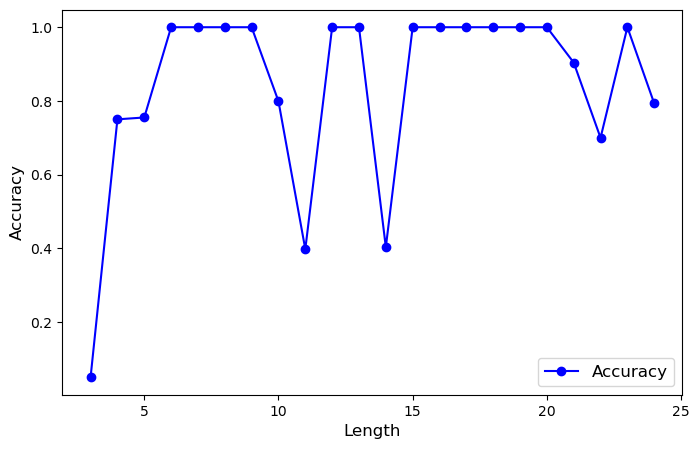
\includegraphics[width=\textwidth]{fig1.png}
        \caption{Experiment result on LSTM.}
        \label{fig:p1}
    \end{minipage}
    \hfill
    \begin{minipage}{0.3\textwidth}
        \centering
        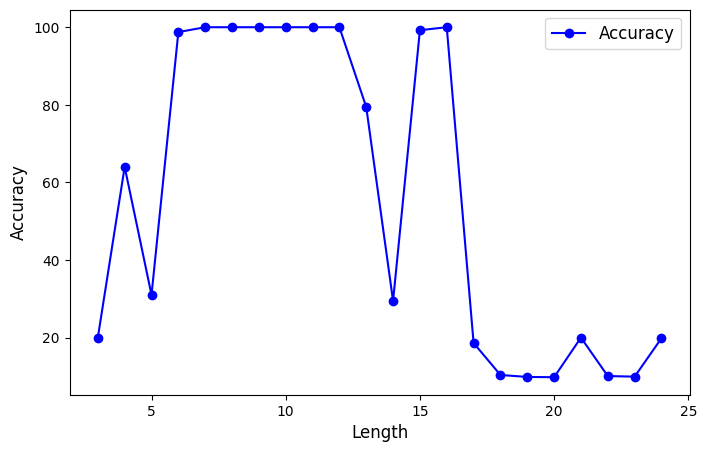
\includegraphics[width=\textwidth]{fig2.png}
        \caption{Experiment result on RNN.}
        \label{fig:p2}
    \end{minipage}
    \hfill
    \begin{minipage}{0.3\textwidth}
        \centering
        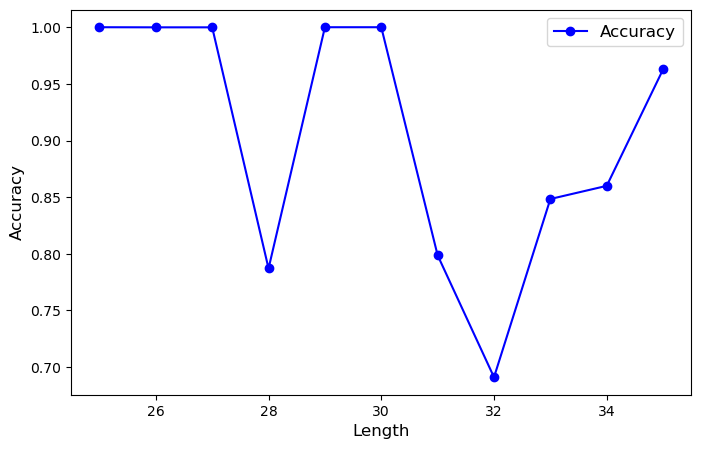
\includegraphics[width=\textwidth]{fig3.png}
        \caption{Extra experiment result on LSTM.}
        \label{fig:p3}
    \end{minipage}
\end{figure}

\section{GAN}

\subsection{Model}

GAN consists of two primary components: a generator and a discriminator, which are trained adversarially.

The Generator (\(G\)) is a neural network designed to map a latent space vector (\(z\)) sampled from a noise distribution to a realistic data distribution. The architecture is as follows:

\begin{itemize}
    \item Input: A latent vector of dimension \(d_{z}\) (default: \(100\)).
    \item Layers:
        \begin{itemize}
            \item Linear layer: Maps \(z \in \mathbb{R}^{d_z}\) to \(128\)-dimensional space.
            \item LeakyReLU activation (\(\alpha=0.2\)).
            \item Linear layer: Expands to \(256\) dimensions, followed by Batch Normalization and LeakyReLU.
            \item Linear layer: Expands to \(512\) dimensions, followed by Batch Normalization and LeakyReLU.
            \item Linear layer: Expands to \(1024\) dimensions, followed by Batch Normalization and LeakyReLU.
            \item Linear layer: Maps \(1024\)-dimensional space to \(784\) (flattened \(28\times28\)) dimensions, followed by a \(tanh\) activation to normalize pixel values to \([-1, 1]\).
        \end{itemize}
    \item Output: A \(784\)-dimensional vector reshaped into a \(28\times28\) image.
\end{itemize}

The Discriminator (\(D\)) is a binary classifier designed to distinguish real images from fake images generated by \(G\). The architecture is:

\begin{itemize}
    \item Input: A flattened \(28\times28 = 784\)-dimensional image vector.
    \item Layers:
        \begin{itemize}
            \item Linear layer: Maps \(784\)-dimensional input to \(512\) dimensions.
            \item LeakyReLU activation (\(\alpha=0.2\)).
            \item Linear layer: Reduces to \(256\) dimensions, followed by LeakyReLU.
            \item Linear layer: Reduces to \(1\) dimension, followed by a Sigmoid activation to produce a probability.
        \end{itemize}
    \item Output: A scalar in \([0, 1]\), representing the likelihood of the input being a real image.
\end{itemize}

\subsection{Training}

The GAN is trained using a min-max optimization objective:

\[
\min_{G} \max_{D} V(D, G) = \mathbb{E}_{x \sim p_{\text{data}}}[\log D(x)] + \mathbb{E}_{z \sim p_z}[\log(1 - D(G(z)))]
\]

\begin{itemize}
    \item Discriminator Training: \(D\) is trained to maximize the likelihood of correctly classifying real and fake images.
  \[
  L_D = - \mathbb{E}_{x \sim p_{\text{data}}}[\log D(x)] - \mathbb{E}_{z \sim p_z}[\log(1 - D(G(z)))]
  \]
    \item Generator Training: \(G\) is trained to minimize \(\log(1 - D(G(z)))\), which is equivalent to maximizing \(\log D(G(z))\).
  \[
  L_G = - \mathbb{E}_{z \sim p_z}[\log D(G(z))]
  \]
\end{itemize}

\subsection{Experiment}

The experiment is conducted on the MNIST dataset. Both \(G\) and \(D\) are trained with an Adam optimizer with learning rate \(0.0002\) for \(200\) epochs. \cref{fig:p4,fig:p5,fig:p6} show the performance of the generator G before, during and after the training.

The experimental results show that the generator can effectively mimic the samples from the dataset. Additionally, we conducted an interpolation experiment with \(7\) steps between two different digits in the latent space. The generated images \cref{fig:p7} in each step not only resemble valid digits but also exhibit a smooth transition effect. These two experiments demonstrate the effectiveness of the trained generator.

\begin{figure}[t]
    \centering
    \begin{minipage}{0.3\textwidth}
        \centering
        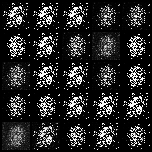
\includegraphics[width=\textwidth]{0.png}
        \caption{\(G\) before training.}
        \label{fig:p4}
    \end{minipage}%
    \hfill
    \begin{minipage}{0.3\textwidth}
        \centering
        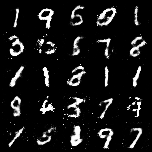
\includegraphics[width=\textwidth]{100.png}
        \caption{\(G\) after training for \(100\) epochs.}
        \label{fig:p5}
    \end{minipage}
    \hfill
    \begin{minipage}{0.3\textwidth}
        \centering
        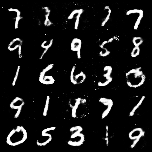
\includegraphics[width=\textwidth]{199.png}
        \caption{\(G\) after training for \(200\) epochs.}
        \label{fig:p6}
    \end{minipage}
\end{figure}

\begin{figure}[t]
    \centering
    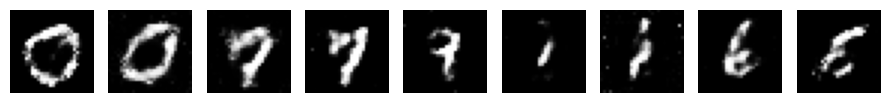
\includegraphics[width=0.5\linewidth]{p7.png}
    \caption{Results of the interpolation experiment.}
    \label{fig:p7}
\end{figure}

% --------------------------------------------------------------
%     You don't have to mess with anything below this line.
% --------------------------------------------------------------
 
\end{document}
